\begin{remark}
    Section made from lectures done by Kjellmar Oksavik. Other sources are \citet{BrekkeAsgeir2013Potu} --- chapter 4 parts 1 to 6. \& chapter 7 parts 6 to 10.
\end{remark}
\section[Production of ionization]{The production of ionization by solar radiation}
When it comes to the composition if the ionosphere, \(\pres{}{}{NO}^+\) and \(\pres{}{}{O}_2^+\) dominate below 150 km, while \(\pres{}{}{O}^+\) dominates a long way above 150 km. Above 300 km it is \(\pres{}{}{H}^+\) that is more important than \(\pres{}{}{NO}^+\) and \(\pres{}{}{O}_2^+\). \(\pres{}{}{O}^+\) may dominate as high as 600 km, but this is strongly dependant on magnetospheric and solar conditions.

\section[The ionization profile]{The ionization profile of the upper atmosphere}
We will assume that the target atmosphere the solar radiation penetrates is a horizontally stratified medium, and that this medium obeys the equation of state for an ideal gas. For an atmospheric gas in hydrostatic equilibrium the particle density will decrease by altitude as
\begin{equation*}
    n=n_0e^{-z/H}
\end{equation*}
where \(H=kT/mg\) is the \(e\)-fold scale height.

Incoming wavelength \(\lambda \) will have an intensity \(I\left(\lambda,z\right)\) at altitude  \(z\). There will be a cross-section \(\sigma\left(\lambda\right)\) for ionization of neutral particles in the atmosphere by radiation at wavelength \(\lambda \). Solar radiation at wavelength \(\lambda \) will therefore ionize a number of neutral particles per cubic meter and second.

If the radiation with intensity \(I(\lambda)\) has passed a distance \(s\) through the atmosphere, the intensity will be reduced by \(\tn{d}I\) if it passes an additional infinitesimal distance \(\tn{d}s\) (\cref{fig:L10_radiation_medium}) through a slab of the atmosphere. This reduction has to be proportional to the intensity of the radiation, the cross-section for ionization, and the number of targets that can be ionized. The reduction of \(I\) per unit distance is as follows
\begin{equation}\label{eq:L10_reduction_of_I}
    \fracd[s]{I}=-n\sigma I
\end{equation}
Let us assume that for every unit energy absorbed of radiation, there will be formed a number \(C\) electrons. Then the production of electrons per cubic meter and second can be expressed as
\begin{equation*}
    q=C\sigma nI=-C\fracd[s]{I}
\end{equation*}
\(C\) is called the ionization efficiency. For atomic species the ionization efficiency \(C\) is unity so all the energy of the radiation goes into producing ion–electron pairs; for molecules, however, \(C<1\).

We now realize that since \(n\) increases and \(I\) decreases as we go down in the atmosphere, the product must reach a maximum somewhere, and this maximum is found where
\begin{equation*}
    \fracd[s]{q}=C\sigma\left(I\fracd[s]{n}+n\fracd[s]{I}\right)=0
\end{equation*}
where \(C\) and \(\sigma \) are constants. By introducing the index \(m\) for maximum we get
\begin{equation}\label{eq:L10_index_m}
    \frac{1}{n_m}{\left(\fracd[s]{n}\right)}_m+\frac{1}{I_m}{\left(\fracd[s]{I}\right)}_m=0
\end{equation}
If radiation falls in towards the atmosphere by an angle \(\chi \) with respect to the zenith, we see that
\begin{equation}\label{eq:L10_ds_rewritten}
    \tn{d}s=-\frac{\tn{d}z}{\cos\chi}
\end{equation}
hence
\begin{equation*}
    \frac{1}{n}\fracd[s]{n}=-\frac{1}{n}\fracd[z]{n}\cos\chi=\frac{\cos\chi}{H}
\end{equation*}
At the maximum we have
\begin{equation*}
    \frac{1}{I_m}{\left(\fracd[s]{I}\right)}_m=-\sigma n_m
\end{equation*}
so going back to \cref{eq:L10_index_m} we can now write
\begin{equation*}
    \frac{\cos\chi}{H}-\sigma n_m=0
\end{equation*}
\begin{equation*}
    \Rightarrow\sigma Hn_m\sec\chi=1
\end{equation*}
We know from earlier that for an atmosphere with a constant scale height
\begin{equation*}
    n_0H=\mathcal{N}
\end{equation*}
where \(\mathcal{N}\) is the total number of particles between the reference height and infinity. At maximum ionization we then get
\begin{equation*}
    Hn_m=\mathcal{N}_m\Rightarrow \sigma \mathcal{N}_m\sec\chi=1
\end{equation*}
where \(\mathcal{N}_m\) is the number of neutral particles above a unit area at height \(z_m\) in the
atmosphere.

Inserting \cref{eq:L10_ds_rewritten} into \cref{eq:L10_reduction_of_I} we find
\begin{equation*}
    \frac{1}{I}\fracd[s]{I}=-\frac{1}{I}\fracd[z]{I}\cos\chi=-\sigma n=-\sigma n_0e^{-\frac{z}{H}}
\end{equation*}
and
\begin{equation*}
    \frac{\tn{d}I}{I}=\sigma n_0e^{-\frac{z}{H}}\sec\chi\tn{d}z
\end{equation*}
For \(z=\infty \), \(I=I_\infty \), that is, at the source of radiation
\begin{equation*}
    \int_{I_\infty}^I\frac{\tn{d}I}{I}=\sigma n_0\sec\chi\int_\infty^{z}e^{-\frac{z}{H}}\tn{d}z
\end{equation*}
and
\begin{equation*}
    \ln\left|\frac{I}{I_\infty}\right|=-\sigma H\sec\chi n(z)
\end{equation*}
\begin{figure}[t]
    \centering
    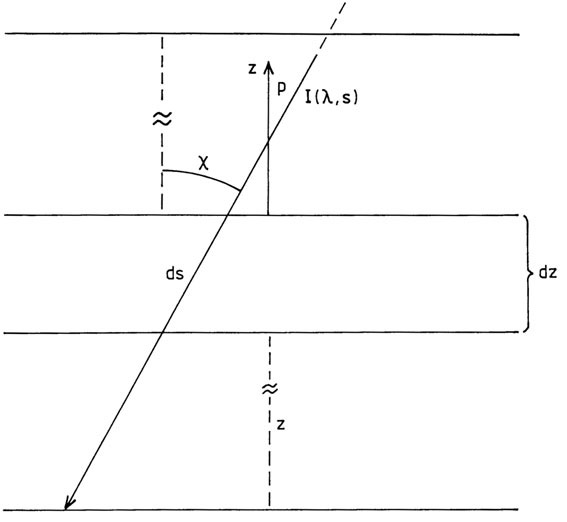
\includegraphics[width=.4\linewidth]{bilder/L10_radiation_medium.jpg}
    \caption{Illustration of the geometry related to solar irradiation (\(I\)) when penetrating a slab of thickness \(\tn{d}z\) in the Earth’s atmosphere at a zenith angle \(\chi \). The distance to the source and to the ground are \(s\) and \(z\), respectively.}\label{fig:L10_radiation_medium}
\end{figure}

At the height of maximum ionization we have
\begin{equation*}
    \ln\left|\frac{I_m}{I_\infty}\right|=-\sigma n_{m}H\sec\chi=-1
\end{equation*}
and
\begin{equation*}
    I_m=\frac{I_\infty}{e}
\end{equation*}
The intensity of the radiation has therefore decreased by \(1/e\) at the height of the ion production maximum. In general, however,
\begin{equation*}
    I=I_\infty e^{-\sigma nH\sec\chi}=I_\infty e^{-\tau}
\end{equation*}
where \(\tau=\sigma nH\sec\chi \) is the optical depth. For the maximum ionization, this optical depth is
\begin{equation*}
    \tau_m=\sigma n_{m}H\sec\chi=\sigma n_0e^{-\frac{z_m}{H}}H\sec\chi=1
\end{equation*}
For an overhead Sun (\(\chi=\SI{0}{\degree}\))
\begin{equation*}
    e^{\frac{z_{m,0}}{H}}=\sigma n_0H \Rightarrow e^{\frac{z_m}{H}}=e^{\frac{z_{m,0}}{H}}\sec\chi
\end{equation*}
and
\begin{equation*}
    \frac{z_m}{H}=\frac{z_{m,0}}{H}+\ln\sec\chi
\end{equation*}
The height of the maximum ion production increases as the zenith angle increases, and the lowest height (\(z_{m,0}\)) it can reach is for overhead Sun. We also found that \(\ln|I/I_m|=-(n-n_m)\sigma H\sec\chi=(1-n/n_m)\), from which we obtain
\begin{equation*}
    \frac{I}{I_m}=e^{\left(1-n/n_m\right)}
\end{equation*}
This shows the relationship between the intensity of the radiation at a given neutral density relative to the intensity and neutral density at the maximum of ionization.

Now, neither the ionization cross-section nor the scale height is constant by altitude, therefore a more correct definition of optical depth would be
\coloredeq{eq:L10_optical_depth}{\tau_\lambda(z)=-\sec\chi\int_\infty^z\sigma_\lambda(z') n (z')\tn{d}z'}
\begin{figure}[t]
    \centering
    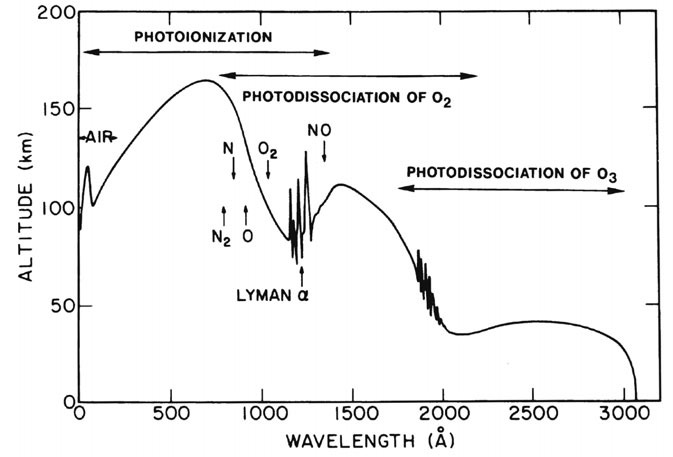
\includegraphics[width=.6\linewidth]{bilder/L10_optical_depth_wavelength.jpg}
    \caption{The altitude of unit optical depth in the wavelength region below \(\num{3000}\si{\angstrom}\). This corresponds to the level where maximum energy is dissipated at each wavelength. The arrows indicate at what wavelength region the most typical ionization and dissociation processes take place. (From Giraud and Petit, 1978.)}\label{fig:L10_optical_depth_wavelength}
\end{figure}

We notice in \cref{fig:L10_optical_depth_wavelength} that there are a few spectral lines that are absorbed very strongly with respect to some neighbor lines, and some lines, especially \(Ly_\alpha \) at 1215 Å, are reaching deeper down in the atmosphere than lines close by in the spectrum. The \(Ly_\alpha \) line, by the way, penetrates all the way down to the D-region where it ionizes \(\pres{}{}{NO}\).

Characteristic threshold energy is given as
\begin{equation*}
    V_p=h\nu=h\frac{c}{\lambda}
\end{equation*}
If the radiation has higher energy than \(V_p\)
\begin{equation*}
    h\nu=V_p+E_\lambda^*+E_e
\end{equation*}
where \(E_\lambda^*\) is an excited ion and \(E_e\) is the kinetic energy of the electron. If \(E_e>V_p\) then we get secondary ionization.

According to laboratory experiments it is found that the mean energy \(\overline{\epsilon}\) lost per impact ionization is almost constant as long as \(E_e\gg V_p\). The total number of free electrons produced per photoionization is then given by
\begin{equation*}
    N=1+\frac{h\nu-\overline{V}_p}{\overline{\epsilon}}
\end{equation*}

\section{Ionization profiles}
The ion production rate at maximum is
\begin{equation*}
    q_m=C\sigma n_m I_m=C\sigma n_m\frac{I_\infty}{e}=\frac{CI_\infty}{eH}\cos\chi
\end{equation*}
and for an overhead Sun we find
\begin{align*}
    q_{m,0}=\frac{CI_\infty}{eH}\\
    \therefore q_m=q_{m,0}\cos\chi
\end{align*}
Production at maximum can never be larger than for an overhead Sun, and it decreases as \(\cos\chi \) for increasing zenith angle \(\chi \).

For ion production rate we can make the ratio
\begin{align}
    \frac{q}{q_m}&=\frac{Cn\sigma I}{Cn_m\sigma I_m}=\frac{n}{n_m}e^{\left(1-\frac{n}{n_m}\right)},\qquad\frac{n}{n_m}=e^{-\frac{z-z_m}{H}}\notag \\
    q&=q_m\exp\left[1-y-\exp\left(-y\right)\right]\label{eq:L10_production_at_height}
\end{align}
where \(y=(z-z_m)/H\).

Inserting \(z_m/H=z_{m,0}/H+\ln\sec\chi \) into \cref{eq:L10_production_at_height} yields
\coloredeq{eq:L10_production_maximum}{\begin{aligned}
    q&=q_m\sec\chi\exp\left[1-x-\sec\chi\exp\left(-x\right)\right]\\
    &=q_{m,0}\exp\left[1-x-\sec\chi\exp\left(-x\right)\right]
\end{aligned}}
where \(x=(z-z_{m,0})/H\). For very large \(x\) (\(z\gg z_{m,0}\)) the profile takes the form
\begin{equation*}
    q\approx q_{m,0}\exp\left(-z/H\right)
\end{equation*}
Well above the maximum in the ionization profile the profile itself decays by altitude as the density of the target atmosphere. This holds for \(x>2\) (i.e.\ at a distance more than two scale heights above \(z_{m,0}\)). This relation arises because at those heights the intensity of the radiation is only weakly reduced, and the rate of production is essentially proportional to the density of the target gas.

For very large negative \(x\) (\(z\ll z_{m,0}\)) the production rate takes the form
\begin{equation*}
    q=q_{m,0}\exp\left[-\sec\chi\exp\left(-x\right)\right]
\end{equation*}
and the profile decreases very rapidly with height below the altitude of peak production.

What we see is that a short wavelength will have its production maximum at a lower altitude, compared to longer wavelengths.

\section{The recombination process}
We here start off at the continuity equation
\begin{equation*}
    \p{t}{n_i}=q_i-\ell_i-\nabla\cdot\left(\gf{v}_{i}n_i\right)
\end{equation*}
where \(n_i\) is the density, \(q_i\) the production, \(\ell_i\) is the loss by chemical and photochemical processes, and the last term is the divergence due to transport phenomena through a volume of interest (the convection term).

\subsection{E-region}
We start by neglecting transport and assume photochemical equilibrium, i.e.~\(q_i=\ell_i\). Let us further assume that electrons \(e\) recombine directly with positive ions \(\pres{}{}{X}^+\) to form a neutral species together with an accompanying radiation of a photon, \(h\nu \)
\begin{equation*}
    \pres{}{}{X}^++e\rightarrow \pres{}{}{X}+h\nu
\end{equation*}
(rate \(10^{-18}\tn{m}^3/\tn{s}\) small) the so-called radiative recombination process. Another possibility for reducing the number of free electrons is by dissociative recombination of a molecule \(\pres{}{}{XY}^+\) as
\begin{equation*}
    \pres{}{}{XY}^++e\rightarrow \pres{}{}{X}+\pres{}{}{Y}
\end{equation*}
(rate \(10^{-13}\tn{m}^3/\tn{s}\) large).

Whether the radiative recombination process or the dissociative recombination process is dominant, we will in both cases for simplicity assume charge neutrality so that the number density of positive ions \([\pres{}{}{X}^+]=n_e\) or \([\pres{}{}{XY}^+]=n_e\) are equal to the number density ne of free electrons. The loss rate will be proportional to
\begin{equation*}
    \ell_i=\alpha \left[\pres{}{}{X}^+\right]n_e=\alpha n_e^2
\end{equation*}
where the proportionality factor \(\alpha \) is called the ``recombination coefficient''. For photochemical equilibrium
\begin{equation*}
    \ell_i=q_i=q_{m,0}\exp\left[1-x-\sec\chi\exp\left(-x\right)\right]=\alpha n_e^2
\end{equation*}
Electron density at a given height \(z\) is therefore
\begin{equation*}
    n_e(z)=\sqrt{\frac{q_{m,0}}{\alpha}}\exp\left[\frac{1}{2}\left(1-x-\sec\chi\exp\left(-x\right)\right)\right]
\end{equation*}
When neglecting height variations of \(\alpha \) we find the maximum of the electron density \(\tn{d}n_e/\tn{d}x=0\) to give us
\begin{equation*}
    e^{-x}=\cos\chi
\end{equation*}
showing that the electron density at maximum is given by
\begin{equation*}
    n_m=\sqrt{\frac{q_{m,0}}{\alpha}\cos\chi}=n_{m,0}\sqrt{\cos\chi}
\end{equation*}
The maximum electron density varies as \(\sqrt{\cos\chi}\) with zenith angle. This is often called a Chapman \(\alpha \)-profile and is representative of the \emph{E-region}.

\subsection{D-region}
If, ont the other hand, electrons are lost by attachment to a molecule
\begin{equation*}
    \pres{}{}{M}+e\rightarrow \pres{}{}{M}^-
\end{equation*}
the the loss rate is proportional to \(n_e\) and can be expressed as
\begin{equation*}
    \ell_i=\beta n_e
\end{equation*}
where \(\beta \) is proportional to \([\pres{}{}{M}]\), the density of the neutral molecule \(\pres{}{}{M}\). In equilibrium
\begin{equation*}
    q_i=\ell_i=\beta n_e
\end{equation*}
and the electron density profile is given by applying \cref{eq:L10_production_maximum}
\begin{equation*}
    n_e=\frac{q_{m,0}}{\beta}\exp\left[1-x-\sec\chi\exp(-x)\right]
\end{equation*}
We again neglect variations in our proportionality factor, now \(\beta \), and again we get for the maximum electron density \(\exp(-x)=\cos\chi \) and
\begin{equation*}
    n_m=\frac{q_{m,0}}{\beta}\cos\chi=n_{m,0}\cos\chi
\end{equation*}
The maximum density varies with the zenith angle as \(\cos\chi \). This is often called a Chapman \(\beta \)-profile and is representative of the \emph{D-region}.

\section{The \(\pres{}{}{O}^+\) dominant ionosphere}
In the F-region above, say, 150 km, the dominant ions formed by solar irradiance are the \(\pres{}{}{O}^+\) (below 150 km \(\pres{}{}{O}_2^+\) and \(\pres{}{}{NO}^+\)).

The atomic oxygen ions when produced can be lost by several reactions. \boxed{\tn{Alternative 1:}}
\begin{equation*}
    \pres{}{}{O}^++e\overset{\alpha_r}{\longrightarrow}\pres{}{}{O}+h\nu\qquad\tn{(slow)}
\end{equation*}
where \(\alpha_r\) is the radiative recombination coefficient. A more rapid loss process for the atomic oxygen is through a chain of reactions. \boxed{\tn{Alternative 2:}}
\begin{align*}
    \pres{}{}{O}^++\pres{}{}{N}_2&\overset{k_1}{\longrightarrow}\pres{}{}{NO}^++\pres{}{}{N}\\
    \pres{}{}{NO}^++e&\overset{\alpha_1}{\longrightarrow}\pres{}{}{N}+\pres{}{}{O}
\end{align*}
where \(\alpha_1\) is the relevant dissociative recombination coefficient. \boxed{\tn{Alternative 3:}}
\begin{align*}
    \pres{}{}{O}^++\pres{}{}{O}_2&\overset{k_2}{\longrightarrow}\pres{}{}{O}_2^++\pres{}{}{O}\\
    \pres{}{}{O}_2^++e&\overset{\alpha_2}{\longrightarrow}\pres{}{}{O}+\pres{}{}{O}
\end{align*}
with a rate coefficient for the process given by \(k_2\), and the dissociative recombination rate given as \(\alpha_2\).

In a quasi-chemical photoequilibrium condition the production of atomic oxygen ions must be equal to the loss of these ions
\begin{equation*}
    q(\pres{}{}{O}^+)=\ell(\pres{}{}{O}^+)=\left(k_1[\pres{}{}{N}_2]+k_2[\pres{}{}{O}_2]\right)[\pres{}{}{O}^+]
\end{equation*}
when we neglect radiative recombination. For molecular oxygen ions we have a similar equilibrium condition when neglecting the production of \(\pres{}{}{O}_2^+\) due to solar radiation
\begin{align*}
    &q(\pres{}{}{O}_2^+)=k_2[\pres{}{}{O}_2][\pres{}{}{O}^+]\\
    &\ell(\pres{}{}{O}_2^+)=\alpha_2 [\pres{}{}{O}_2^+]n_e
\end{align*}
and since \(q(\pres{}{}{O}_2^+)=\ell(\pres{}{}{O}_2^+)\)
\begin{equation}\label{eq:L10_production_O_2}
    [\pres{}{}{O}_2^+]=\frac{k_2}{\alpha_2}\frac{[\pres{}{}{O}_2]}{n_e}[\pres{}{}{O}^+]
\end{equation}
and for the \(\pres{}{}{NO}^+\) ions when no solar production is assumed
\begin{align*}
    &q\left(\pres{}{}{NO}^+\right)=k_1[\pres{}{}{O}^+][\pres{}{}{N}_2]\\
    &\ell\left(\pres{}{}{NO}^+\right)=\alpha_1 [\pres{}{}{NO}^+]n_e
\end{align*}
and since \(q\left(\pres{}{}{NO}^+\right)=\ell\left(\pres{}{}{NO}^+\right)\)
\begin{equation}\label{eq:L10_production_NO}
    [\pres{}{}{NO}^+]=\frac{k_1}{\alpha_2}\frac{[\pres{}{}{N}_2]}{n_e}[\pres{}{}{O}^+]
\end{equation}

Since the number of positive and negative charges must be equal we have
\begin{equation*}
    n_e=[\pres{}{}{O}^+]+[\pres{}{}{NO}^+]+[\pres{}{}{O}_2^+]
\end{equation*}
and plugging in from \cref{eq:L10_production_O_2,eq:L10_production_NO} we get
\begin{equation*}
    n_e=\left(1+\frac{k_1}{\alpha_1}\frac{[\pres{}{}{N}_2]}{n_e}+\frac{k_2}{\alpha_2}\frac{[\pres{}{}{O}_2]}{n_e}\right)[\pres{}{}{O}^+]
\end{equation*}
Solving for \([\pres{}{}{O}^+]\) we can obtain
\begin{equation*}
    q(\pres{}{}{O}^+)=\left(\frac{k_1[\pres{}{}{N}_2]+k_2[\pres{}{}{O}_2]}{1+\frac{k_1}{\alpha_1}\frac{[\pres{}{}{N}_2]}{n_e}+\frac{k_2}{\alpha_2}\frac{[\pres{}{}{O}_2]}{n_e}}\right)n_e=\beta'n_e
\end{equation*}
where \(\beta'\) is the loss rate. The values for \(k_1\) and \(k_2\) are of order \(\num{2e-18}\tn{m}^3\tn{s}\), while \(\alpha_1\) and \(\alpha_2\) are of the order of \(\num{1e-13}\tn{m}^3\tn{s}\). For altitudes above 250 km or so where \([\pres{}{}{N}_2]<10^{15}\tn{m}^{-3}\) and \([\pres{}{}{O}_2]\approx 10^{14}\tn{m}^{-3}\), we get an electron density of the order of \(n_e\sim 10^{11}\tn{m}^{-3}\). Since \(\pres{}{}{N}_2\) and \(\pres{}{}{O}_2\) have similar scale heights above 250 km, it is a good approximation to set
\begin{equation}
    \beta\approx\beta_0\exp\left[-\frac{z-z_0}{H}\right]
\end{equation}
where \(\beta_0\) is the effective loss rate at \(z_0\).

If we go to the lower F-region and the E-region, the reactions involving charge rearrangement between \(\pres{}{}{O}^+\) and \(\pres{}{}{O}_2\) and \(\pres{}{}{N}_2\) will become more abundant because of the increase in molecular neutral
density and, therefore, the complete expression for \(\beta'\) must be maintained.

Solving for \(n_e\) we get
\begin{equation*}
    n_e=\frac{q(\pres{}{}{O}^+)}{\beta'}=q(\pres{}{}{O}^+)\frac{1+\left(\frac{k_1}{\alpha_1}[\pres{}{}{N}_2]+\frac{k_2}{\alpha_2}[\pres{}{}{O}_2]\right)\frac{1}{n_e}}{\beta}
\end{equation*}
We simplify this by writing
\coloredeq{eq:L10_electron_densiy_knee}{n_e=q (\pres{}{}{O}^+)\left[\frac{1}{\beta}+\frac{1}{\alpha_{\tn{eff}}n_e}\right]}
where
\begin{equation*}
    \frac{1}{\alpha_{\tn{eff}}}=\left[\frac{k_1}{\alpha_1}[\pres{}{}{N}_2]+\frac{k_2}{\alpha_2}[\pres{}{}{O}_2]\right]\frac{1}{\beta}
\end{equation*}
Since \(\beta \) decreases by height and \(\alpha_{\tn{eff}}n_e\) will increase by height under F-region maximum, there can be a transition height \(z_t\) at which \(n_e=n_{et}\) and where
\begin{equation*}
    \beta_t=\alpha_{\tn{eff}}n_{et}
\end{equation*}
Above this height the electron density will vary as \(n_e\sim q/\beta \). Below, we have \(n_e\sim\sqrt{q/\alpha_{\tn{eff}}}\).

We have seen from \cref{eq:L10_production_maximum} that for distances larger than two scale heights above the ionization maximum, the ion production profile decays by altitude with the scale height of the background atmosphere (i.e., with the scale height of the oxygen atoms, \(H_{\pres{}{}{O}}\)), since these are the major ionization targets above the F-region peak. We then have
\begin{equation*}
    q(z)\approx\exp\left(-\frac{z}{H_{\pres{}{}{O}}}\right)
\end{equation*}
Since \(\beta \) is proportional to \(k_1[\pres{}{}{N}_2]+k_2[\pres{}{}{O}_2]\), it decays by altitude as the density of \(\pres{}{}{N}_2\) and \(\pres{}{}{O}_2\). As \(\pres{}{}{N}_2\) is the dominant species of the two, we assume
\begin{equation*}
    \beta(z)\approx\exp\left(-\frac{z}{H_{\pres{}{}{N}_2}}\right)
\end{equation*}
The electron density profile at the topside ionosphere therefore will vary according to the following expression
\begin{equation*}
    n_e(z)=\frac{q(z)}{\beta(z)}\propto \exp\left(-\frac{z}{H_O}\right)\exp\left(-\frac{z}{H_{\pres{}{}{N}_2}}\right)=\exp\left[\left(\frac{H_{\pres{}{}{O}}}{H_{\pres{}{}{N}_2}}-1\right)\frac{z}{H_{\pres{}{}{O}}}\right]
\end{equation*}
Since \(H_{\pres{}{}{O}}/H_{\pres{}{}{N}_2}=7/4\) we find
\begin{equation*}
    n_e(z)\propto\exp\left(\frac{3z}{4H_{\pres{}{}{O}}}\right)
\end{equation*}
The electron density profile above the F-region peak will increase by a scale height of \(1.33H_{\pres{}{}{O}}\) if the ionosphere is in photochemical equilibrium. If our assumptions were appropriate for all regions, the electron density would therefore increase to infinity above the altitude \(z_t\).

\section{Ambipolar diffusion}
The ionosphere is simply not in photochemical equilibrium above the F-region peak, and we have to turn our attention to diffusion to see what that can do to the problem.

Let us assume charge neutrality (\(n_e=n_i\)), that the neutral air is in rest (\(\gf{u}=0\)), and that no current is present (\(\gf{v}_i=\gf{v}_e=\gf{v}\)). Since the mass of ions is so much greater than the mass of electrons, a charge separation will occur due to the gravity field which creates an electric field. This field, however, will exert a strong force on electrons compared with gravity and the charge separation will be blocked. In particular, for the vertical motion we will have
\begin{equation*}
    w_i=w_e=w
\end{equation*}
For now, we will also assume no magnetic field and an isothermal plasma in thermal balance with the neutrals (\(T_e=T_i=T_n=T\)).

The momentum equation in the vertical direction for the ions and electrons is
\begin{align*}
    n_{i}m_i\p{t}{w_i}=-\p{z}{}p_i-n_{i}m_{i}g+n_{i}eE-n_{i}m_i\nu_{i}w_i=0\\
    n_{e}m_e\p{t}{w_e}=-\p{z}{}p_e-n_{e}m_{e}g-n_{e}eE-n_{e}m_e\nu_{e}w_e=0
\end{align*}
where \(\nu \) is the collision frequency with neutrals. Any collisions between electrons and ions are neglected. We add the two together and leave the collision terms on the LHS, hence
\begin{equation*}
    n_e\left(m_i\nu_i+m_e\nu_e\right)w=-\p{z}{\left(p_i+p_e\right)}-n_e\left(m_i+m_e\right)g
\end{equation*}
We assume that the ideal gas law applies for the plasma and that \(T\) is constant by height. Simplifying using \(m_i\gg m_e\) and solving for the vertical particle flux \(n_{e}w\) gives
\begin{equation}\label{eq:L10_plasma_diffusion}
    n_{e}w=-\frac{2kT}{\left(m_i\nu_i+m_e\nu_e\right)}\left(\p{z}{n_e}+\frac{n_{e}m_{i}g}{2kT}\right)
\end{equation}
with the equivalent for neutrals being
\begin{equation*}%\label{eq:L10_neutral_gas_diffusion}
    n_{e}w=-\frac{kT}{m\nu}\left(\p{z}{n_e}+\frac{n_{e}m_{i}g}{kT}\right)
\end{equation*}
The scale height of the plasma is
\begin{equation*}
    H_p=\frac{2kT}{m_{i}g}=2H
\end{equation*}
where \(H\) is the scale height of the neutral atmosphere. The plasma diffusion coefficient will be given as
\begin{equation}\label{eq:L10_plasma_diffusion_coefficient}
    D_p=\frac{2kT}{m_i\nu_i+m_e\nu_e}\approx 2D
\end{equation}
where \(m_i\nu_i\gg m_e\nu_e\) and \(D\) is the diffusion coefficient of the neutral gas, and \(D_p\) is often called the \emph{ambipolar diffusion coefficient} referring to the polarization field between ions and electrons which forces the plasma to move as a whole.

The equation of diffusion will be
\begin{equation*}
    \p{t}{n_e}=-\p{z}{}\left(n_{e}w\right)=\p{z}{}\left \{D_p\left(\p{z}{n_e}+\frac{n_e}{H_p}\right)\right \}
\end{equation*}
Equilibrium can be achieved if
\begin{equation*}
    \p{z}{n_e}=-\frac{n_e}{H_p}
\end{equation*}
or
\begin{equation*}
    n_e=n_{e_0}\exp\left(-\frac{z-z_0}{H_p}\right)
\end{equation*}
The equilibrium profile of the electron density will therefore be exponential and decay by altitude with a scale height that is twice as large as the scale height of the neutral atmosphere, where the difference is due to diffusion.

Since the diffusion coefficient for \(m_i\nu_i\gg m_e\nu_e\) is \cref{eq:L10_plasma_diffusion_coefficient} it will decrease exponentially as
\begin{equation*}
    D_p=D_0\exp\left(\frac{z}{H}\right)
\end{equation*}

If \(T_e\neq T_i\) and \(T_e=cT_i\) where \(c\) is some constant, the plasma scale height would be
\begin{equation*}
    H_p=(1+c)H
\end{equation*}
and the plasma diffusion coefficient would be
\begin{equation*}
    D_p=(1+c)D
\end{equation*}
The shape of the profile and the effect of diffusion therefore is strongly dependent
on the electron–ion temperature ratio.